\section{Vordefiniertes Stylesheet}

Das vordefinierte Stylesheet befindet sich im Ordner "`\textbf{default}"' unter Packages. Auf diesem Stylesheet aufbauend kann die Beschreibung der Quests und Packages erstellt werden. Abbildung \ref{fig:defaut_stylesheet} zeigt Beispiele für diese Klassen.

Dieses ist vor allem auf bestimmte Anwendungsgebiete zugeschnitten:
\begin{itemize}
\item Um Codes zu kennzeichnen, kann die Klasse \textit{\textbf{code}} verwendet werden. Diese umrahmt die Auswahl mit gepunkteten Linien.
\item Informationen werden mit der Klasse \textit{\textbf{info}} gekennzeichnet und diese werden mit einer gelben Hintergrundfarbe dargestellt.
\item Fragen haben einen blauen Hintergrund und werden mithilfe der Klasse \textit{\textbf{question}} angesprochen.
\item Duch einen roten Hintergrund kann eine Warnung dargestellt werden. Diese kann anhand der Klasse \textit{\textbf{warning}} verwendet werden.
\end{itemize}

\begin{figure}[h] 
  \centering
     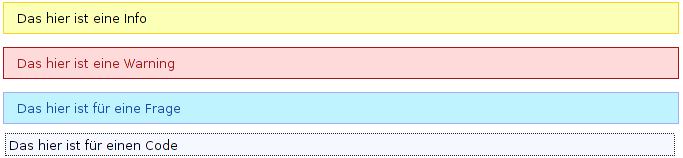
\includegraphics[width=0.9\textwidth]{./media/images/quest/style.png}
  \caption{Beispielhafte Beschreibung}
  \label{fig:defaut_stylesheet}
\end{figure}